\section{CAD第十三次作业}
\setcounter{subsection}{0}
\subsection{题目:}

\tt{仿真确认：在端口加压求流，确认正反馈的差分对是一个N型负阻}

\tt{仿真确认：N型负阻并联在并联LC谐振腔中，可形成正弦振荡（电容两端电压）}

\tt{当电容很小，谐振腔Q值很小时，正弦振荡退化为张弛振荡}

\begin{figure}[!ht]
\centering
\resizebox{0.8\textwidth}{!}{%
\begin{circuitikz}
\tikzstyle{every node}=[font=\large]
\draw (5,7.5) to[Tnpn, transistors/scale=1.19] (5,10.5);
\draw (8.5,7.5) to[Tnpn, transistors/scale=1.19] (8.5,10.5);
\draw (4,9) to[short] (4,11.5);
\draw (4,11.5) to[short] (8.5,11.5);
\draw (8.5,10.5) to[short] (8.5,13);
\draw (7.5,9) to[short] (7.5,10.5);
\draw (5,10.5) to[short] (7.5,10.5);
\draw (5,7.5) to[short] (5,6.75);
\draw (8.5,7.5) to[short] (8.5,6.75);
\draw (5,6.75) to[short] (8.5,6.75);
\draw (2.75,7.75) to[american current source,l={ \large $0.5I_{EE}$}] (2.75,10.75);
\draw (10.75,8) to[american current source,l={ \large $0.5I_{EE}$}] (10.75,11.25);
\draw (2.75,10.5) to[short] (2.75,13.5);
\draw (5,10.5) to[short] (5,13.75);
\draw (2.75,13.25) to[short] (2.75,13.75);
\draw (2.75,13.75) to[short] (5,13.75);
\draw (8.5,12.5) to[short] (8.5,13.75);
\draw (10.75,11) to[short] (10.75,13.75);
\draw (8.5,13.75) to[short] (10.75,13.75);
\draw (10.75,8.5) to[short] (10.75,6.75);
\draw (2.75,8) to[short] (2.75,6.75);
\draw (2.75,6.75) to[short] (10.75,6.75);
\draw (2.75,6.75) to (2.75,6) node[ground]{};
\node [font=\large] at (6.75,14) {$$};
\node [font=\large] at (9.5,12.75) {$$};
\node at (8.5,11.5) [circ] {};
\node at (5,10.5) [circ] {};
\end{circuitikz}
}%

\label{fig:my_label}
\end{figure}

\begin{figure}[H]
\centering
\resizebox{0.8\textwidth}{!}{%
\begin{circuitikz}
\tikzstyle{every node}=[font=\large]
\draw (5,7.5) to[Tnpn, transistors/scale=1.19] (5,10.5);
\draw (8.5,7.5) to[Tnpn, transistors/scale=1.19] (8.5,10.5);
\draw (4,9) to[short] (4,11.5);
\draw (4,11.5) to[short] (8.5,11.5);
\draw (8.5,10.5) to[short] (8.5,13);
\draw (7.5,9) to[short] (7.5,10.5);
\draw (5,10.5) to[short] (7.5,10.5);
\draw (5,7.5) to[short] (5,6.75);
\draw (8.5,7.5) to[short] (8.5,6.75);
\draw (5,6.75) to[short] (8.5,6.75);
\draw (2.75,7.75) to[american current source,l={ \large $0.5I_{EE}$}] (2.75,10.75);
\draw (10.75,8) to[american current source,l={ \large $0.5I_{EE}$}] (10.75,11.25);
\draw (2.75,10.5) to[short] (2.75,13.5);
\draw (5,10.5) to[short] (5,13.75);
\draw (2.75,13.25) to[short] (2.75,13.75);
\draw (2.75,13.75) to[short] (5,13.75);
\draw (8.5,12.5) to[short] (8.5,13.75);
\draw (10.75,11) to[short] (10.75,13.75);
\draw (8.5,13.75) to[short] (10.75,13.75);
\draw (10.75,8.5) to[short] (10.75,6.75);
\draw (2.75,8) to[short] (2.75,6.75);
\draw (2.75,6.75) to[short] (10.75,6.75);
\draw (2.75,6.75) to (2.75,6) node[ground]{};
\node [font=\large] at (6.75,14) {$$};
\node [font=\large] at (9.5,12.75) {$$};
\node at (8.5,11.5) [circ] {};
\node at (5,10.5) [circ] {};
\draw (5,12.5) to[C,l={ \large $C$}] (8.5,12.5);
\draw (5,13.75) to[L,l={ \large $L/2$} ] (6.5,13.75);
\draw (7,13.75) to[L,l={ \large $L/2$} ] (8.5,13.75);
\draw (6.5,13.75) to[short] (7,13.75);
\draw (6.75,13.75) to[short, -o] (6.75,14.75) ;
\end{circuitikz}
}%

\label{fig:my_label}
\end{figure}
\subsection{N型负阻的仿真确认:}

\begin{figure}[H]
\centering
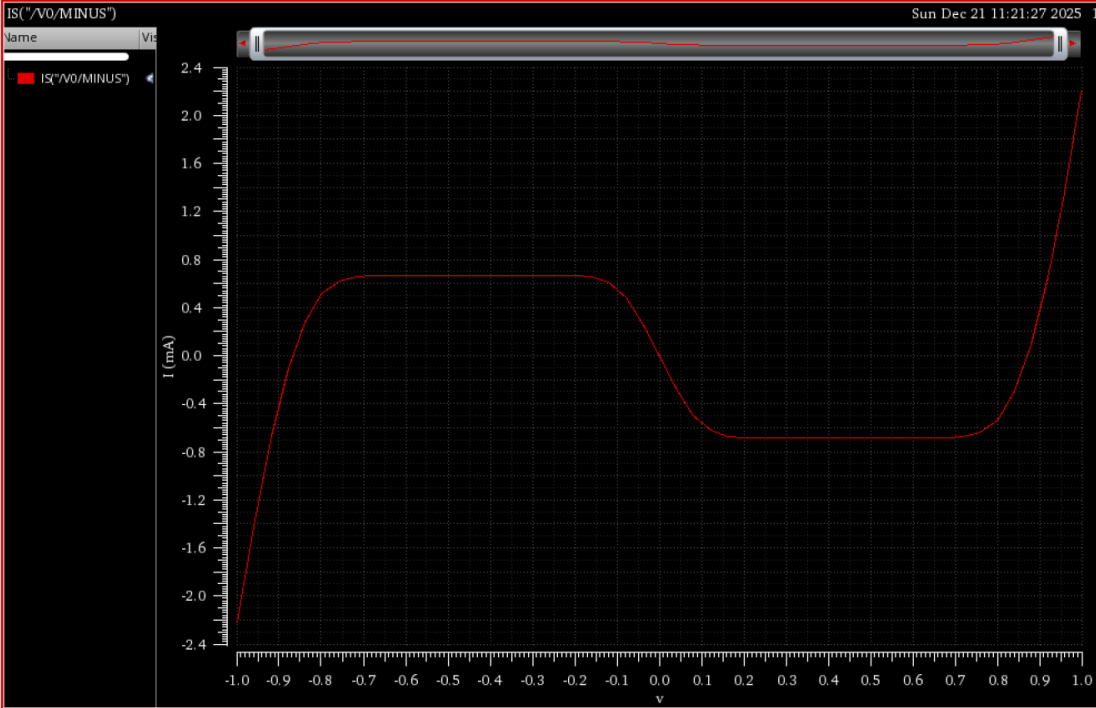
\includegraphics[width=0.8\textwidth]{chapters/figure/A28/N.png}
\caption{N型负阻的仿真结果:在端口加压求流，确认正反馈的差分对是一个N型负阻}
\label{fig:my_label}
\end{figure}

\tt{可以看出，在端口加压求流的仿真结果中，正反馈的差分对表现出N型负阻的特性。这意味着在某些电压范围内，电流会随着电压的增加而减少，形成负阻现象。}

\subsection{正弦振荡的仿真确认:}

\begin{figure}[!ht]
\centering
\resizebox{0.3\textwidth}{!}{%
\begin{circuitikz}
\tikzstyle{every node}=[font=\large]
\draw (5,7.5) to[Tnpn, transistors/scale=1.19] (5,10.5);
\draw (8.5,7.5) to[Tnpn, transistors/scale=1.19] (8.5,10.5);
\draw (4,9) to[short] (4,11.5);
\draw (4,11.5) to[short] (8.5,11.5);
\draw (8.5,10.5) to[short] (8.5,13);
\draw (7.5,9) to[short] (7.5,10.5);
\draw (5,10.5) to[short] (7.5,10.5);
\draw (5,7.5) to[short] (5,6.75);
\draw (8.5,7.5) to[short] (8.5,6.75);
\draw (5,6.75) to[short] (8.5,6.75);
\draw (5,10.5) to[short] (5,13.75);
\draw (8.5,12.5) to[short] (8.5,13.75);
\node [font=\large] at (6.75,14) {$$};
\node [font=\large] at (9.5,12.75) {$$};
\node at (8.5,11.5) [circ] {};
\node at (5,10.5) [circ] {};
\draw (5,12.5) to[C,l={ \large $1uF$}] (8.5,12.5);
\draw (5,13.75) to[L,l={ \large $500pH$} ] (6.5,13.75);
\draw (7,13.75) to[L,l={ \large $500pH$} ] (8.5,13.75);
\draw (6.5,13.75) to[short] (7,13.75);
\draw (6.75,13.75) to[short, -o] (6.75,14.75) ;
\draw (6.75,6.75) to[american current source,l={ \large $100uA$}] (6.75,5);
\draw (6.75,5) to (6.75,4.75) node[ground]{};
\end{circuitikz}
}%

\label{fig:my_label}
\end{figure}

\begin{figure}[!ht]
\centering
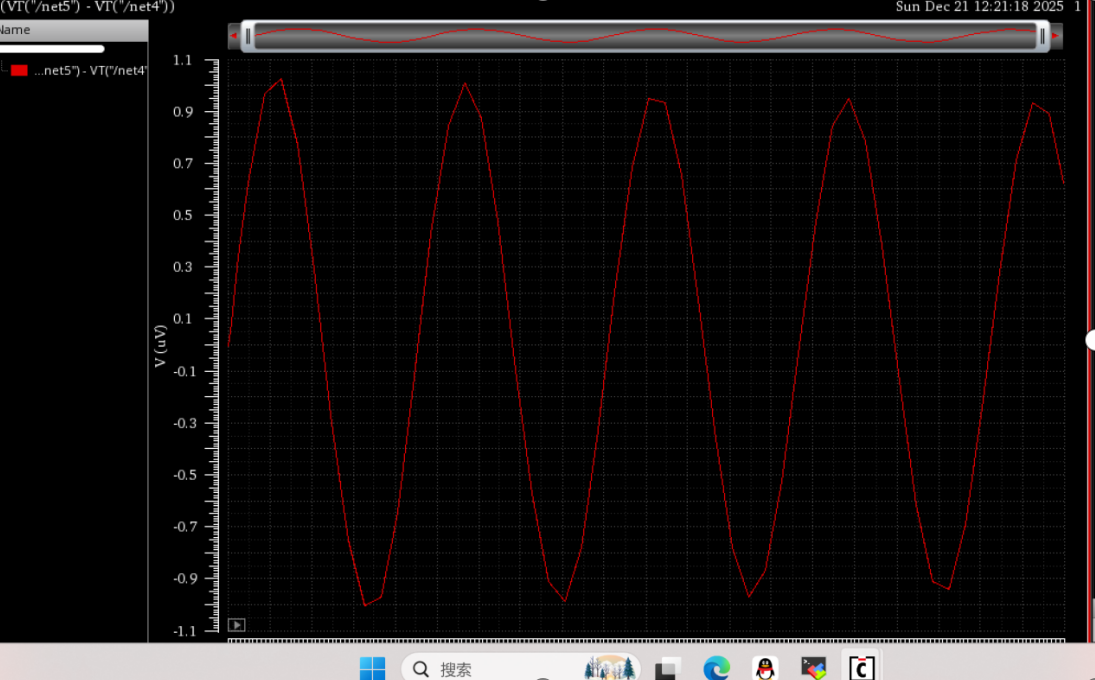
\includegraphics[width=0.8\textwidth]{chapters/figure/A28/震荡.png}
\caption{正弦振荡的仿真结果: N型负阻并联在并联LC谐振腔中，可形成正弦振荡（电容两端电压）}
\label{zhendang}
\end{figure}

\tt{从图\ref{zhendang}可以看出，在N型负阻并联在并联LC谐振腔中的仿真结果中，电容两端的电压表现出正弦振荡的特性。这表明该电路能够形成稳定的正弦振荡，验证了N型负阻在谐振腔中的作用。}

\subsection{张弛振荡的仿真确认:}

\begin{figure}[!ht]
\centering
\resizebox{0.3\textwidth}{!}{%
\begin{circuitikz}
\tikzstyle{every node}=[font=\large]
\draw (5,7.5) to[Tnpn, transistors/scale=1.19] (5,10.5);
\draw (8.5,7.5) to[Tnpn, transistors/scale=1.19] (8.5,10.5);
\draw (4,9) to[short] (4,11.5);
\draw (4,11.5) to[short] (8.5,11.5);
\draw (8.5,10.5) to[short] (8.5,13);
\draw (7.5,9) to[short] (7.5,10.5);
\draw (5,10.5) to[short] (7.5,10.5);
\draw (5,7.5) to[short] (5,6.75);
\draw (8.5,7.5) to[short] (8.5,6.75);
\draw (5,6.75) to[short] (8.5,6.75);
\draw (5,10.5) to[short] (5,13.75);
\draw (8.5,12.5) to[short] (8.5,13.75);
\node [font=\large] at (6.75,14) {$$};
\node [font=\large] at (9.5,12.75) {$$};
\node at (8.5,11.5) [circ] {};
\node at (5,10.5) [circ] {};
\draw (5,12.5) to[C,l={ \large $1uF$}] (8.5,12.5);
\draw (5,13.75) to[L,l={ \large $500nH$} ] (6.5,13.75);
\draw (7,13.75) to[L,l={ \large $500nH$} ] (8.5,13.75);
\draw (6.5,13.75) to[short] (7,13.75);
\draw (6.75,13.75) to[short, -o] (6.75,14.75) ;
\draw (6.75,6.75) to[american current source,l={ \large $100uA$}] (6.75,5);
\draw (6.75,5) to (6.75,4.75) node[ground]{};
\end{circuitikz}
}%

\label{fig:my_label}
\end{figure}

\begin{figure}[!ht]
\centering
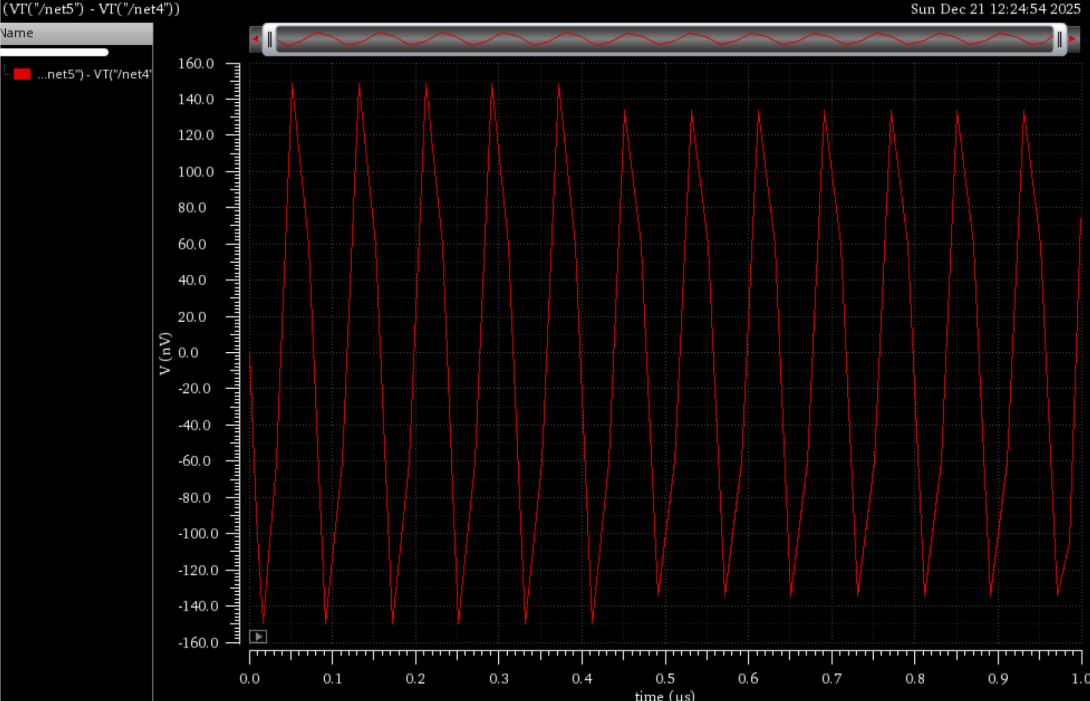
\includegraphics[width=0.8\textwidth]{chapters/figure/A28/张弛.png}
\caption{张弛振荡的仿真结果: 当电容很小，谐振腔Q值很小时，正弦振荡退化为张弛振荡}
\label{zhangchi}
\end{figure}

\tt{从图\ref{zhangchi}可以看出，当电容很小且谐振腔Q值很小时，电容两端的电压表现出张弛振荡的特性。这表明在这种条件下，正弦振荡退化为张弛振荡，验证了电路参数对振荡类型的影响。}

